%-----------------------------------------------------------------------------------------
% Autor dieser Vorlage:
% Stefan Macke (http://fachinformatiker-anwendungsentwicklung.net)
% Permalink zur Vorlage: http://fiae.link/LaTeXVorlageFIAE
%
% Sämtliche verwendeten Abbildungen, Tabellen und Listings stammen von Dirk Grashorn.
%
% Lizenz: Creative Commons 4.0 Namensnennung - Weitergabe unter gleichen Bedingungen
% -----------------------------------------------------------------------------------------

\documentclass[
	ngerman,
	toc=listof, % Abbildungsverzeichnis sowie Tabellenverzeichnis in das Inhaltsverzeichnis aufnehmen
	toc=bibliography, % Literaturverzeichnis in das Inhaltsverzeichnis aufnehmen
	footnotes=multiple, % Trennen von direkt aufeinander folgenden Fußnoten
	parskip=half, % vertikalen Abstand zwischen Absätzen verwenden anstatt horizontale Einrückung von Folgeabsätzen
	numbers=noendperiod % Den letzten Punkt nach einer Nummerierung entfernen (nach DIN 5008)
]{scrartcl}
\pdfminorversion=5 % erlaubt das Einfügen von pdf-Dateien bis Version 1.7, ohne eine Fehlermeldung zu werfen (keine Garantie für fehlerfreies Einbetten!)
\usepackage[utf8]{inputenc} % muss als erstes eingebunden werden, da Meta/Packages ggfs. Sonderzeichen enthalten

% !TEX root = Projektdokumentation.tex

% Hinweis: der Titel muss zum Inhalt des Projekts passen und den zentralen Inhalt des Projekts deutlich herausstellen
\newcommand{\titel}{Entwicklung von NatInfo}
\newcommand{\untertitel}{Webbasiertes Tool zur Unterstützung der Entwickler}
\newcommand{\kompletterTitel}{\titel{} -- \untertitel}

\newcommand{\autorName}{Stefan Macke}
\newcommand{\autorAnschrift}{Meine Straße 1}
\newcommand{\autorOrt}{49377 Vechta}

\newcommand{\betriebLogo}{LogoBetrieb.pdf}
\newcommand{\betriebName}{\textsc{Alte Oldenburger} Krankenversicherung AG}
\newcommand{\betriebAnschrift}{Theodor-Heuss-Str. 96}
\newcommand{\betriebOrt}{49377 Vechta}

\newcommand{\ausbildungsberuf}{Fachinformatiker für Anwendungsentwicklung}
\newcommand{\betreff}{Dokumentation zur betrieblichen Projektarbeit}
\newcommand{\pruefungstermin}{Sommer 2015}
\newcommand{\abgabeOrt}{Vechta}
\newcommand{\abgabeTermin}{23.04.2015}
 % Metadaten zu diesem Dokument (Autor usw.)
% !TEX root = ../Projektdokumentation.tex

% Anpassung an Landessprache ---------------------------------------------------
\usepackage{babel}

% Umlaute ----------------------------------------------------------------------
%   Umlaute/Sonderzeichen wie äüöß direkt im Quelltext verwenden (CodePage).
%   Erlaubt automatische Trennung von Worten mit Umlauten.
% ------------------------------------------------------------------------------
\usepackage[T1]{fontenc}
\usepackage{textcomp} % Euro-Zeichen etc.

% Schrift ----------------------------------------------------------------------
\usepackage{lmodern} % bessere Fonts
\usepackage{relsize} % Schriftgröße relativ festlegen

% Tabellen ---------------------------------------------------------------------
\PassOptionsToPackage{table}{xcolor}
\usepackage{tabularx}
% für lange Tabellen
\usepackage{longtable}
\usepackage{array}
\usepackage{ragged2e}
\usepackage{lscape}
\newcolumntype{w}[1]{>{\raggedleft\hspace{0pt}}p{#1}} % Spaltendefinition rechtsbündig mit definierter Breite

% Grafiken ---------------------------------------------------------------------
\usepackage[dvips,final]{graphicx} % Einbinden von JPG-Grafiken ermöglichen
\usepackage{graphics} % keepaspectratio
\usepackage{floatflt} % zum Umfließen von Bildern
\graphicspath{{Bilder/}} % hier liegen die Bilder des Dokuments

% Sonstiges --------------------------------------------------------------------
\usepackage[titles]{tocloft} % Inhaltsverzeichnis DIN 5008 gerecht einrücken
\usepackage{amsmath,amsfonts} % Befehle aus AMSTeX für mathematische Symbole
\usepackage{enumitem} % anpassbare Enumerates/Itemizes
\usepackage{xspace} % sorgt dafür, dass Leerzeichen hinter parameterlosen Makros nicht als Makroendezeichen interpretiert werden

\usepackage{makeidx} % für Index-Ausgabe mit \printindex
\usepackage[printonlyused]{acronym} % es werden nur benutzte Definitionen aufgelistet

% Einfache Definition der Zeilenabstände und Seitenränder etc.
\usepackage{setspace}
\usepackage{geometry}

% Symbolverzeichnis
\usepackage[intoc]{nomencl}
\let\abbrev\nomenclature
\renewcommand{\nomname}{Abkürzungsverzeichnis}
\setlength{\nomlabelwidth}{.25\hsize}
\renewcommand{\nomlabel}[1]{#1 \dotfill}
\setlength{\nomitemsep}{-\parsep}

\usepackage{varioref} % Elegantere Verweise. „auf der nächsten Seite“
\usepackage{url} % URL verlinken, lange URLs umbrechen etc.

\usepackage{chngcntr} % fortlaufendes Durchnummerieren der Fußnoten
% \usepackage[perpage]{footmisc} % Alternative: Nummerierung der Fußnoten auf jeder Seite neu

\usepackage{ifthen} % bei der Definition eigener Befehle benötigt
\usepackage{todonotes} % definiert u.a. die Befehle \todo und \listoftodos
\usepackage[square]{natbib} % wichtig für korrekte Zitierweise

% PDF-Optionen -----------------------------------------------------------------
\usepackage{pdfpages}
\pdfminorversion=5 % erlaubt das Einfügen von pdf-Dateien bis Version 1.7, ohne eine Fehlermeldung zu werfen (keine Garantie für fehlerfreies Einbetten!)
\usepackage[
    bookmarks,
    bookmarksnumbered,
    bookmarksopen=true,
    bookmarksopenlevel=1,
    colorlinks=true,
% diese Farbdefinitionen zeichnen Links im PDF farblich aus
    anchorcolor=AOBlau,% Ankertext
    citecolor=AOBlau, % Verweise auf Literaturverzeichniseinträge im Text
    filecolor=AOBlau, % Verknüpfungen, die lokale Dateien öffnen
    menucolor=AOBlau, % Acrobat-Menüpunkte
    urlcolor=AOBlau,
% diese Farbdefinitionen sollten für den Druck verwendet werden (alles schwarz)
    %linkcolor=black, % einfache interne Verknüpfungen
    %anchorcolor=black, % Ankertext
    %citecolor=black, % Verweise auf Literaturverzeichniseinträge im Text
    %filecolor=black, % Verknüpfungen, die lokale Dateien öffnen
    %menucolor=black, % Acrobat-Menüpunkte
    %urlcolor=black,
%
    %backref, % Quellen werden zurück auf ihre Zitate verlinkt
    pdftex,
    plainpages=false, % zur korrekten Erstellung der Bookmarks
    pdfpagelabels=true, % zur korrekten Erstellung der Bookmarks
    hypertexnames=false, % zur korrekten Erstellung der Bookmarks
    linkcolor=black,
    linktoc=all,
]{hyperref}
% Befehle, die Umlaute ausgeben, führen zu Fehlern, wenn sie hyperref als Optionen übergeben werden
\hypersetup{
    pdftitle={\titel -- \untertitel},
    pdfauthor={\autorName},
    pdfcreator={\autorName},
    pdfsubject={\titel -- \untertitel},
    pdfkeywords={\titel -- \untertitel},
}


% zum Einbinden von Programmcode -----------------------------------------------
\usepackage{listings}
\usepackage{xcolor}
\definecolor{hellgelb}{rgb}{1,1,0.9}
\definecolor{colKeys}{rgb}{0,0,1}
\definecolor{colIdentifier}{rgb}{0,0,0}
\definecolor{colComments}{rgb}{0,0.5,0}
\definecolor{colString}{rgb}{1,0,0}
\lstset{
    float=hbp,
	basicstyle=\footnotesize,
    identifierstyle=\color{colIdentifier},
    keywordstyle=\color{colKeys},
    stringstyle=\color{colString},
    commentstyle=\color{colComments},
    backgroundcolor=\color{hellgelb},
    columns=flexible,
    tabsize=2,
    frame=single,
    extendedchars=true,
    showspaces=false,
    showstringspaces=false,
    numbers=left,
    numberstyle=\tiny,
    breaklines=true,
    breakautoindent=true,
	captionpos=b,
}
\lstdefinelanguage{cs}{
	sensitive=false,
	morecomment=[l]{//},
	morecomment=[s]{/*}{*/},
	morestring=[b]",
	morekeywords={
		abstract,event,new,struct,as,explicit,null,switch
		base,extern,object,this,bool,false,operator,throw,
		break,finally,out,true,byte,fixed,override,try,
		case,float,params,typeof,catch,for,private,uint,
		char,foreach,protected,ulong,checked,goto,public,unchecked,
		class,if,readonly,unsafe,const,implicit,ref,ushort,
		continue,in,return,using,decimal,int,sbyte,virtual,
		default,interface,sealed,volatile,delegate,internal,short,void,
		do,is,sizeof,while,double,lock,stackalloc,
		else,long,static,enum,namespace,string},
}
\lstdefinelanguage{natural}{
	sensitive=false,
	morecomment=[l]{/*},
	morestring=[b]",
	morestring=[b]',
	alsodigit={-,*},
	morekeywords={
		DEFINE,DATA,LOCAL,END-DEFINE,WRITE,CALLNAT,PARAMETER,USING,
		IF,NOT,END-IF,ON,*ERROR-NR,ERROR,END-ERROR,ESCAPE,ROUTINE,
		PERFORM,SUBROUTINE,END-SUBROUTINE,CONST,END-FOR,END,FOR,RESIZE,
		ARRAY,TO,BY,VALUE,RESET,COMPRESS,INTO,EQ},
}
\lstdefinelanguage{php}{
	sensitive=false,
	morecomment=[l]{/*},
	morestring=[b]",
	morestring=[b]',
	alsodigit={-,*},
	morekeywords={
		abstract,and,array,as,break,case,catch,cfunction,class,clone,const,
		continue,declare,default,do,else,elseif,enddeclare,endfor,endforeach,
		endif,endswitch,endwhile,extends,final,for,foreach,function,global,
		goto,if,implements,interface,instanceof,namespace,new,old_function,or,
		private,protected,public,static,switch,throw,try,use,var,while,xor
		die,echo,empty,exit,eval,include,include_once,isset,list,require,
		require_once,return,print,unset},
}
 % verwendete Packages
% !TEX root = ../Projektdokumentation.tex

% Seitenränder -----------------------------------------------------------------
\setlength{\topskip}{\ht\strutbox} % behebt Warnung von geometry
\geometry{a4paper,left=20mm,right=20mm,top=25mm,bottom=35mm}

\usepackage[
	automark, % Kapitelangaben in Kopfzeile automatisch erstellen
	headsepline, % Trennlinie unter Kopfzeile
	ilines % Trennlinie linksbündig ausrichten
]{scrlayer-scrpage}

% Kopf- und Fußzeilen ----------------------------------------------------------
\pagestyle{scrheadings}
% chapterpagestyle gibt es nicht in scrartcl
%\renewcommand{\chapterpagestyle}{scrheadings}
\clearscrheadfoot

% Kopfzeile
\renewcommand{\headfont}{\normalfont} % Schriftform der Kopfzeile
\ihead{\large{\textsc{\titel}}\\ \small{\untertitel} \\[2ex] \textit{\headmark}}
\chead{}
\ohead{\includegraphics[scale=0.4]{\betriebLogo}}
\setlength{\headheight}{15mm} % Höhe der Kopfzeile
%\setheadwidth[0pt]{textwithmarginpar} % Kopfzeile über den Text hinaus verbreitern (falls Logo den Text überdeckt)

% Fußzeile
\ifoot{\autorName}
\cfoot{}
\ofoot{\pagemark}

% Überschriften nach DIN 5008 in einer Fluchtlinie
% ------------------------------------------------------------------------------

% Abstand zwischen Nummerierung und Überschrift definieren
% > Schön wäre hier die dynamische Berechnung des Abstandes in Abhängigkeit
% > der Verschachtelungstiefe des Inhaltsverzeichnisses
\newcommand{\headingSpace}{1.5cm}

% Abschnittsüberschriften im selben Stil wie beim Inhaltsverzeichnis einrücken
\renewcommand*{\othersectionlevelsformat}[3]{
  \makebox[\headingSpace][l]{#3\autodot}
}

% Für die Einrückung wird das Paket tocloft benötigt
%\cftsetindents{chapter}{0.0cm}{\headingSpace}
\cftsetindents{section}{0.0cm}{\headingSpace}
\cftsetindents{subsection}{0.0cm}{\headingSpace}
\cftsetindents{subsubsection}{0.0cm}{\headingSpace}
\cftsetindents{figure}{0.0cm}{\headingSpace}
\cftsetindents{table}{0.0cm}{\headingSpace}


% Allgemeines
% ------------------------------------------------------------------------------

\onehalfspacing % Zeilenabstand 1,5 Zeilen
\frenchspacing % erzeugt ein wenig mehr Platz hinter einem Punkt

% Schusterjungen und Hurenkinder vermeiden
\clubpenalty = 10000
\widowpenalty = 10000
\displaywidowpenalty = 10000

% Quellcode-Ausgabe formatieren
\lstset{numbers=left, numberstyle=\tiny, numbersep=5pt, breaklines=true}
\lstset{emph={square}, emphstyle=\color{red}, emph={[2]root,base}, emphstyle={[2]\color{blue}}}

\counterwithout{footnote}{section} % Fußnoten fortlaufend durchnummerieren
\setcounter{tocdepth}{3} % im Inhaltsverzeichnis werden die Kapitel bis zum Level der subsubsection übernommen
\setcounter{secnumdepth}{3} % Kapitel bis zum Level der subsubsection werden nummeriert

% Aufzählungen anpassen
\renewcommand{\labelenumi}{\arabic{enumi}.}
\renewcommand{\labelenumii}{\arabic{enumi}.\arabic{enumii}.}
\renewcommand{\labelenumiii}{\arabic{enumi}.\arabic{enumii}.\arabic{enumiii}}

% Tabellenfärbung:
\definecolor{heading}{rgb}{0.64,0.78,0.86}
\definecolor{odd}{rgb}{0.9,0.9,0.9}
 % Definitionen zum Aussehen der Seiten
% !TEX root = ../Projektdokumentation.tex

% Abkürzungen, ggfs. mit korrektem Leerraum
\newcommand{\bs}{$\backslash$\xspace}
\newcommand{\bspw}{bspw.\xspace}
\newcommand{\bzw}{bzw.\xspace}
\newcommand{\ca}{ca.\xspace}
\newcommand{\dahe}{\mbox{d.\,h.}\xspace}
\newcommand{\etc}{etc.\xspace}
\newcommand{\eur}[1]{\mbox{#1\,\texteuro}\xspace}
\newcommand{\evtl}{evtl.\xspace}
\newcommand{\ggfs}{ggfs.\xspace}
\newcommand{\Ggfs}{Ggfs.\xspace}
\newcommand{\gqq}[1]{\glqq{}#1\grqq{}}
\newcommand{\inkl}{inkl.\xspace}
\newcommand{\insb}{insb.\xspace}
\newcommand{\ua}{\mbox{u.\,a.}\xspace}
\newcommand{\usw}{usw.\xspace}
\newcommand{\Vgl}{Vgl.\xspace}
\newcommand{\zB}{\mbox{z.\,B.}\xspace}

% Befehle für häufig anfallende Aufgaben
\newcommand{\Abbildung}[1]{\autoref{fig:#1}}
\newcommand{\Anhang}[1]{\appendixname{}~\ref{#1}: \nameref{#1} \vpageref{#1}}
\newcommand{\includegraphicsKeepAspectRatio}[2]{\includegraphics[width=#2\textwidth,height=#2\textheight,keepaspectratio]{#1}}
\newcommand{\Zitat}[2][\empty]{\ifthenelse{\equal{#1}{\empty}}{\citep{#2}}{\citep[#1]{#2}}}
\newcommand{\Autor}[1]{\textsc{#1}} % zum Ausgeben von Autoren
\newcommand{\itemd}[2]{\item{\textbf{#1}}\\{#2}} % erzeugt ein Listenelement mit fetter Überschrift

% fügt Tabellen aus einer TEX-Datei ein
\newcommand{\tabelle}[3] % Parameter: caption, label, file
{\begin{table}[htbp]
\centering
\singlespacing
\input{Tabellen/#3}
\caption{#1}
\label{#2}
\end{table}}

\newcommand{\tabelleAnhang}[1] % Parameter: file
{\begin{center}
\singlespacing
\input{Tabellen/#1}
\end{center}}

% einfaches Wechseln der Schrift, z.B.: \changefont{cmss}{sbc}{n}
\newcommand{\changefont}[3]{\fontfamily{#1} \fontseries{#2} \fontshape{#3} \selectfont}

% Verwendung analog zu \includegraphics
\newlength{\myx} % Variable zum Speichern der Bildbreite
\newlength{\myy} % Variable zum Speichern der Bildhöhe
\newcommand\includegraphicstotab[2][\relax]{%
% Abspeichern der Bildabmessungen
\settowidth{\myx}{\includegraphics[{#1}]{#2}}%
\settoheight{\myy}{\includegraphics[{#1}]{#2}}%
% das eigentliche Einfügen
\parbox[c][1.1\myy][c]{\myx}{%
\includegraphics[{#1}]{#2}}%
}

\definecolor{AOBlau}{rgb}{0, 0.28, 0.56}

% verschiedene Befehle um Wörter semantisch auszuzeichnen ----------------------
\newcommand{\Index}[2][\empty]{\ifthenelse{\equal{#1}{\empty}}{\index{#2}#2}{\index{#1}#2}}
\newcommand{\Fachbegriff}[2][\empty]{\ifthenelse{\equal{#1}{\empty}}{\textit{\Index{#2}}}{\textit{\Index[#1]{#2}}}}
\newcommand{\NeuerBegriff}[2][\empty]{\ifthenelse{\equal{#1}{\empty}}{\textbf{\Index{#2}}}{\textbf{\Index[#1]{#2}}}}

\newcommand{\Ausgabe}[1]{\texttt{#1}}
\newcommand{\Eingabe}[1]{\texttt{#1}}
\newcommand{\Code}[1]{\texttt{#1}}
\newcommand{\Datei}[1]{\texttt{#1}}

\newcommand{\Assembly}[1]{\textsf{#1}}
\newcommand{\Klasse}[1]{\textsf{#1}}
\newcommand{\Methode}[1]{\textsf{#1}}
\newcommand{\Attribut}[1]{\textsf{#1}}

\newcommand{\Datentyp}[1]{\textsf{#1}}
\newcommand{\XMLElement}[1]{\textsf{#1}}
\newcommand{\Webservice}[1]{\textsf{#1}}

\newcommand{\Refactoring}[1]{\Fachbegriff{#1}}
\newcommand{\CodeSmell}[1]{\Fachbegriff{#1}}
\newcommand{\Metrik}[1]{\Fachbegriff{#1}}
\newcommand{\DesignPattern}[1]{\Fachbegriff{#1}}
 % eigene allgemeine Befehle, die z.B. die Arbeit mit LaTeX erleichtern
% Abkürzungen
\newcommand{\Versis}{\textsc{Versis}\xspace}
\newcommand{\NI}{NatInfo\xspace}
\newcommand{\AO}{\textsc{Alte Oldenburger} Krankenversicherung\xspace}
 % eigene projektspezifische Befehle, z.B. Abkürzungen usw.

\begin{document}

% kann nach dem Lesen entfernt werden ---------------------------------------
% \pagestyle{plain}
% % !TEX root = Projektdokumentation.tex
\section*{Über diese Vorlage}

Diese \LaTeX-Vorlage wurde von Stefan Macke\footnote{Blog des Autors:
\url{http://fachinformatiker-anwendungsentwicklung.net}, Twitter:
\Eingabe{@StefanMacke}} als Grundlage für die Projektdokumentationen der Auszubildenden zum Fachinformatiker mit Fachrichtung
Anwendungsentwicklung bei der \AO entwickelt. Nichtsdestotrotz dürfte sie ebenso für die anderen IT-Berufe\footnote{\zB IT-Kaufleute, Fachinformatiker
mit Fachrichtung Systemintegration \usw} geeignet sein, da diese anhand der gleichen Verordnung bewertet werden.

Diese Vorlage enthält bereits eine Vorstrukturierung der möglichen Inhalte einer tatsächlichen Projektdokumentation, die auf Basis der
Erfahrungen im Rahmen der Prüfertätigkeit des Autors erstellt und unter Zuhilfenahme von \citet{Rohrer2011} abgerundet wurden.

Sämtliche verwendeten Abbildungen, Tabellen und Listings stammen von \citet{Grashorn2010}.

Download-Link für diese Vorlage: \url{http://fiae.link/LaTeXVorlageFIAE}

Auch verfügbar auf GitHub: \url{https://github.com/StefanMacke/latex-vorlage-fiae}

\subsection*{Lizenz}

\begin{center}
\includegraphicsKeepAspectRatio{CC-Logo.pdf}{0.3}
\end{center}
Dieses Werk steht unter einer Creative Commons Namensnennung - Weitergabe unter gleichen Bedingungen 4.0 International Lizenz.
\footnote{\url{http://creativecommons.org/licenses/by-sa/4.0/}}

\begin{center}
\includegraphicsKeepAspectRatio{CC-Attribution.pdf}{0.07}
\includegraphicsKeepAspectRatio{CC-ShareAlike.pdf}{0.07}
\end{center}

\begin{description}
	\item[Namensnennung] Sie müssen den Namen des Autors/Rechteinhabers in der von ihm festgelegten Weise nennen.
	\footnote{Die Namensnennung im \LaTeX-Quelltext mit Link auf \url{http://fiae.link/LaTeXVorlageFIAE} reicht hierfür aus.}
	\item[Weitergabe unter gleichen Bedingungen] Wenn Sie das lizenzierte Werk \bzw den lizenzierten Inhalt bearbeiten
	oder in anderer Weise erkennbar als Grundlage für eigenes Schaffen verwenden, dürfen Sie die daraufhin neu entstandenen
	Werke \bzw Inhalte nur unter Verwendung von Lizenzbedingungen weitergeben, die mit denen dieses Lizenzvertrages identisch oder vergleichbar sind.
\end{description}

\subsection*{Inhalt der Projektdokumentation}

Grundsätzlich definiert die \citet[S.~1746]{Bundesgesetzblatt48}\footnote{Dieses
Dokument sowie alle weiteren hier genannten können unter
\url{http://fiae.link/LaTeXVorlageFIAEQuellen} heruntergeladen werden.} das Ziel der Projektdokumentation wie folgt:
\begin{quote}
"`Durch die Projektarbeit und deren Dokumentation soll der Prüfling belegen, daß er Arbeitsabläufe und Teilaufgaben zielorientiert unter
Beachtung wirtschaftlicher, technischer, organisatorischer und zeitlicher Vorgaben selbständig planen und kundengerecht umsetzen sowie
Dokumentationen kundengerecht anfertigen, zusammenstellen und modifizieren kann."'
\end{quote}

Und das \citet[S.~36]{BMBF2000} ergänzt:
\begin{quote}
"`Die Ausführung der Projektarbeit wird mit praxisbezogenen Unterlagen dokumentiert.
Der Prüfungsausschuss bewertet die Projektarbeit anhand der Dokumentation. Dabei
wird nicht das Ergebnis -- \zB ein lauffähiges Programm -- herangezogen, sondern
der Arbeitsprozess. Die Dokumentation ist keine wissenschaftliche Abhandlung,
sondern eine handlungsorientierte Darstellung des Projektablaufs mit
praxisbezogenen, d.h. betriebüblichen Unterlagen. Sie soll einen Umfang von
maximal 10 bis 15 DIN A 4-Seiten nicht überschreiten. Soweit erforderlich können in
einem Anhang \zB den Zusammenhang erläuternde Darstellungen beigefügt werden."'
\end{quote}

Außerdem werden dort die grundlegenden Inhalte der Projektdokumentation aufgelistet:
\begin{itemize}
	\item Name und Ausbildungsberuf des Prüfungsteilnehmers
	\item Angabe des Ausbildungsbetriebes
	\item Thema der Projektarbeit
	\item Falls erforderlich, Beschreibung/Konkretisierung des Auftrages
	\item Umfassende Beschreibung der Prozessschritte und der erzielten Ergebnisse
	\item Gegebenenfalls Veränderungen zum Projektantrag mit Begründung
	\item Wenn für das Projekt erforderlich, ein Anhang mit praxisbezogenen Unterlagen und Dokumenten. Dieser Anhang sollte nicht
	aufgebläht werden. Die angehängten Dokumente und Unterlagen sind auf das absolute Minimum zu beschränken.
\end{itemize}

In den folgenden Kapiteln werden diese geforderten Inhalte und sinnvolle Ergänzungen nun meist stichwortartig und \ggfs mit
Beispielen beschrieben. Nicht alle Kapitel müssen in jeder Dokumentation vorhanden sein. Handelt es sich \bspw um ein in sich
geschlossenes Projekt, kann das Kapitel~\ref{sec:Projektabgrenzung}: \nameref{sec:Projektabgrenzung} entfallen; arbeitet die
Anwendung nur mit \acs{XML}-Dateien, kann und muss keine Datenbank beschrieben werden \usw


\subsection*{Formale Vorgaben}

Die formalen Vorgaben zum Umfang und zur Gestaltung der Projektdokumentation können je nach IHK recht unterschiedlich sein.
Normalerweise sollte die zuständige IHK einen Leitfaden bereitstellen, in dem alle Formalien nachgelesen werden können,
wie \zB bei der \citet{MerkblattIHK}.

Als Richtwert verwende ich 15 Seiten für den reinen Inhalt. Also in dieser Vorlage alle Seiten, die arabisch nummeriert
sind (ohne das Literaturverzeichnis und die eidesstattliche Erklärung).
Große Abbildungen, Quelltexte, Tabellen \usw gehören in den Anhang, der 25 Seiten nicht überschreiten sollte.

Typographische Konventionen, Seitenränder \usw können in der Datei \Datei{Seitenstil.tex} beliebig angepasst werden.


\subsection*{Bewertungskriterien}
Die Bewertungskriterien für die Benotung der Projektdokumentation sind recht einheitlich und können leicht in Erfahrung
gebracht werden, \zB bei der \citet{BewertungsmatrikIHK}.
Grundsätzlich sollte die Projektdokumentation nach der Fertigstellung noch einmal im Hinblick auf diese Kriterien durchgeschaut werden.

% \cleardoublepage
% \pagestyle{scrheadings}
% ---------------------------------------------------------------------------

\phantomsection
\thispagestyle{plain}
\pdfbookmark[1]{Deckblatt}{deckblatt}
% !TEX root = Projektdokumentation.tex
\begin{titlepage}

\begin{center}

\includegraphics[scale=0.25]{LogoIHK.pdf}\\[1ex]
\Large{Abschlussprüfung \pruefungstermin}\\[3ex]

\Large{\ausbildungsberuf}\\
\LARGE{\betreff}\\[4ex]

\huge{\textbf{\titel}}\\[1.5ex]
\Large{\textbf{\untertitel}}\\[4ex]

\normalsize
Abgabetermin: \abgabeOrt, den \abgabeTermin\\[3em]
\textbf{Prüfungsbewerber:}\\
\autorName\\
\autorAnschrift\\
\autorOrt\\[5ex]

\includegraphics[scale=1]{\betriebLogo}\\[2ex]
\textbf{Ausbildungsbetrieb:}\\
\betriebName\\
\betriebAnschrift\\
\betriebOrt\\[5em]
\end{center}

\small
\noindent
Dieses Werk einschließlich seiner Teile ist \textbf{urheberrechtlich geschützt}.
Jede Verwertung außerhalb der engen Grenzen des Urheberrechtgesetzes ist ohne
Zustimmung des Autors unzulässig und strafbar. Das gilt insbesondere für
Vervielfältigungen, Übersetzungen, Mikroverfilmungen sowie die Einspeicherung
und Verarbeitung in elektronischen Systemen.

\end{titlepage}
\cleardoublepage

% Preface --------------------------------------------------------------------
\phantomsection
\pagenumbering{Roman}
\pdfbookmark[1]{Inhaltsverzeichnis}{inhalt}
\tableofcontents

\cleardoublepage

\phantomsection
\listoffigures
\cleardoublepage

\phantomsection
\listoftables
\cleardoublepage

\newcommand{\abkvz}{Abkürzungsverzeichnis}
\renewcommand{\nomname}{\abkvz}
\section*{\abkvz}
\markboth{\abkvz}{\abkvz}
\addcontentsline{toc}{section}{\abkvz}
% !TEX root = Projektdokumentation.tex

% Es werden nur die Abkürzungen aufgelistet, die mit \ac definiert und auch benutzt wurden. 
%
% \acro{VERSIS}{Versicherungsinformationssystem\acroextra{ (Bestandsführungssystem)}}
% Ergibt in der Liste: VERSIS Versicherungsinformationssystem (Bestandsführungssystem)
% Im Text aber: \ac{VERSIS} -> Versicherungsinformationssystem (VERSIS)

% Hinweis: allgemein bekannte Abkürzungen wie z.B. bzw. u.a. müssen nicht ins Abkürzungsverzeichnis aufgenommen werden
% Hinweis: allgemein bekannte IT-Begriffe wie Datenbank oder Programmiersprache müssen nicht erläutert werden,
%          aber ggfs. Fachbegriffe aus der Domäne des Prüflings (z.B. Versicherung)

% Die Option (in den eckigen Klammern) enthält das längste Label oder
% einen Platzhalter der die Breite der linken Spalte bestimmt.
\begin{acronym}[WWWWW]
	\acro{AO}{\textsc{Alte Oldenburger} Krankenversicherung AG}
	\acro{API}{Application Programming Interface}
	\acro{CSS}{Cascading Style Sheets}
	\acro{CSV}{Comma Separated Value}
	\acro{EPK}{Ereignisgesteuerte Prozesskette}
	\acro{ERM}{En\-ti\-ty-Re\-la\-tion\-ship-Mo\-dell}
	\acro{HTML}{Hypertext Markup Language}\acused{HTML}
	\acro{IDE}{Integrated Development Environment}
	\acro{MVC}[MVC]{Model View Controller}
	\acro{NatInfo}[\textsc{NatInfo}]{Natural Information System}
	\acro{Natural}[\textsc{Natural}]{Programmiersprache der Software AG}\acused{Natural}
	\acro{ORM}{Object-Relational Mapping}
	\acro{PHP}{Hypertext Preprocessor}
	\acro{SDK}{Software Development Kit}
	\acro{SQL}{Structured Query Language}
	\acro{SVN}{Subversion}
	\acro{UML}{Unified Modeling Language}
	\acro{XML}{Extensible Markup Language}
\end{acronym}

\clearpage

% Inhalt ---------------------------------------------------------------------
\pagenumbering{arabic}
% !TEX root = Projektdokumentation.tex
% !TEX root = ../Projektdokumentation.tex
\section{Einleitung}
\label{sec:Einleitung}
Diese Projektdokumentation schildert den Ablauf meines Abschlussprojektes, das ich im Rahmen meiner Ausbildung zum Fachinformatiker für Anwendungsentwicklung durchgeführt habe. Mein Ausbildungsbetrieb ist die form4 GmbH \& Co. KG aus Berlin.

\subsection{Projektumfeld} 
\label{sec:Projektumfeld}
1996 als Internetagentur gegründet hat die form4 GmbH \& Co. KG sich zu einem Softwareunternehmen entwickelt. Die Schwerpunkte liegen auf der Herstellung von Websites und Portalen sowie der Realisierung individueller, webbasierter Softwarelösungen für mittelständische Unternehmen und Organisationen. Das Unternehmen setzt sich aus zwei Abteilungen - im Folgenden als Units bezeichnet - zusammen. Die Web-Unit und die Enterprise-Unit. Der Auftraggeber dieses Projekts ist der Fachbereich TYPO3 bestehend aus den Seniorentwicklern der Web-Unit.

\paragraph{Die Web-Unit}
Schwerpunkt der Webunit ist die technische Umsetzung von Websites und Portalen im öffentlich zugänglichen Bereich. Hierunter fallen auch Community- und eCommerce-Lösungen.

Kerntechnologien sind hierbei PHP, HTML, CSS und JavaScript.

Die meisten von der Webunit realisierten Projekte basieren auf leistungsfähigen Content Management Systemen wie TYPO3 oder Drupal.

\paragraph{Die Enterprise-Unit}
Die Enterprise-Unit beschäftigt sich in erster Linie mit javabasierten Softwaresystemen. Das beinhaltet Intranet- und Unternehmensportale wie auch klassische individuelle datenverwaltende Software und Workflowsysteme.


\subsection{Projektziel} 
\label{sec:Projektziel}
Ziel des Projektes ist die Entwicklung einer TYPO3-Extension (Backend) und dem dazugehörigen Frontend. Diese Extension soll produktiv in Kundenprojekten zum Einsatz kommen und bestehende Implementierungen ablösen. Dadurch sollen Entwickler zukünftig entlastet werden und eine einfache und einheitliche Lösung zur Verwaltung von Datei-Uploads geschaffen werden. 

Des Weiteren soll die Extension in das öffentliche TYPO3 Extension Repository (TER) deployed und der Source-Code auf GitHub mit einer Open Source Lizenz veröffentlicht werden. 


\subsection{Projektbegründung} 
\label{sec:Projektbegruendung}
Die Motivation dieses Projektes ist es, ein einheitliches, einfach zu integrierendes, konfigurierendes und erweiterndes Tool zum Verwalten von asynchronen Dateiuploads zu schaffen. Durch die zentrale und modular gestaltete Konfigurationsschnittstelle soll der Aufwand und die Fehleranfälligkeit bei der Implementierung eines Dateiuploads deutlich reduziert werden.


\subsection{Projektschnittstellen} 
\label{sec:Projektschnittstellen}
Da es sich um eine TYPO3 Extension handelt, verwendet das Projekt dementsprechend intern die APIs die von TYPO3 zur Verfügung gestellt werden. TYPO3 ist ein Open Source Enterprise Content Management System (CMS) für die Umsetzung von kleinen bis hin zu sehr großen multinationalen Websites. Nach außen stellt das Projekt sowohl im Backend als auch im Frontend für die Entwickler eine API bereit, mit der es in ein Kundenprojekt integriert werden kann. Unter anderen die Konfigurationsschnittstelle, mit der zentral die Konfigurationen verwaltet werden.


\subsection{Projektabgrenzung} 
\label{sec:Projektabgrenzung}
Nicht teil dieses Projektes ist die Umsetzung einer GUI bestehend aus HTML, CSS und JavaScript, welches Änderungen am DOM vornimmt. Es werden lediglich die benötigten HTML Formular-Felder erzeugt, mit denen der Benutzer Dateien auswählen kann und die Daten beim Absenden des Formulars an das Backend gesendet werden. Das JavaScript beschränkt sich nur auf die Verarbeitung und Validierung der Daten und stellt eine API bereit, mit deren Hilfe dann jeweils eine ansprechende und Projektspezifische GUI umgesetzt werden kann.

% !TEX root = ../Projektdokumentation.tex
\section{Projektplanung} 
\label{sec:Projektplanung}


\subsection{Projektphasen}
\label{sec:Projektphasen}
Für die Umsetzung des Projektes standen 70 Stunden zur Verfügung, die im Vorfeld in unterschiedliche Projektphasen eingeteilt wurden. Diese können der Tabelle~\ref{tab:Zeitplanung}: Grobe Zeitplanung entnommen werden. Eine detailliertere Zeitplanung findet sich im \Anhang{app:Zeitplanung}. 


\tabelle{Grobe Zeitplanung}{tab:Zeitplanung}{ZeitplanungKurz}

\subsection{Abweichungen vom Projektantrag}
\label{sec:AbweichungenProjektantrag} 

Einige Abweichungen bestehen in der Zeitplanung, da während der Antragstellung die Anforderungen an das Projekt noch nicht klar definiert waren und dementsprechend die Planung nur sehr grob ausfiel. Nach der Anforderungsanalyse und mithilfe des Lastenheftes konnte die Planung deutlich genauer vorgenommen werden. Außerdem wurde auf die Erstellung eines Pflichtenhefts wurde verzichtet, da auf basis des Lastenheftes und der Entwürfe bereits hinreichend Informationen für die Implementierung zur Verfügung standen. Inhaltlich stimmt das Projekt ansonsten mit dem Projektantrag überein. Desweiteren wird vorerst darauf verzichtet, das Projekt nach Abschluss als Open Source Projekt zu veröffentlichen und in das \ac{TER} zu deployen. Dies soll in einem der folgenden Meilensteine verwirklicht werden. 


\subsection{Ressourcenplanung}
\label{sec:Ressourcenplanung}

Zur Umsetzung des Projektes wurden Hardware-, Software und Personalressourcen benötigt. Eine Aufstellung der verwendeten Ressourcen findet sich im \Anhang{app:Ressourcen}. Bei den verwendeten Bibliotheken wurde stets darauf geachtet, dass diese kostenfrei unter einer Open Source Lizenz verfügbar sind, damit anfallende Kosten möglichst gering gehalten werden und das fertige Tool ohne Lizenzprobleme in Kundenprojekte integriert werden kann.


\subsection{Entwicklungsprozess}
\label{sec:Entwicklungsprozess}

Da die Anforderungen an das Projekt klar und überschaubar sind, eignet sich dafür ein einfaches Wasserfallmodell. Anhand der Zeitplanung (\Anhang{app:Zeitplanung}) konnten im Ticketsystem die entsorechenden Tickets angelgt und abgearbeitet werden.

% !TEX root = ../Projektdokumentation.tex
\section{Analysephase} 
\label{sec:Analysephase}


\subsection{Ist-Analyse} 
\label{sec:IstAnalyse}

Im Rahmen mehrerer Kundenprojekte wurden bereits verschiedene Tools, sowohl Open Source als auch kommerziell, für das Hochladen von Dateien evaluiert und eingesetzt. Sowohl Backend- als auch Frontendseitig hat sich bisher allerdings keine zufriedenstellende Lösung ergeben. Gründe gehen von fehlenden Features bis unzureichenden Dokumentationen, unregelmäßige Wartungen und schlechte Anpassbarkeit im Backend und Frontend. 

Backendseitig ist meist auch die Integration in das TYPO3 Ökosystem sehr aufwändig oder muss jedes Mal neu entwickelt werden, was zusätzliche Arbeit und kosten bedeutet. Dazu kommen Security Issues und mangelnde Umsetzung der PSR-Standards.  

Frontendseitig haben sich die bisher getesteten Tools als sehr konfigurationslastig und schlecht anpassbar herausgestellt. Zudem erfolgt die Konfiguration von Backend und Frontend getrennt, was Redundanzen verursacht und zu Inkonsistenzen führen kann. 


\subsection{Wirtschaftlichkeitsanalyse}
\label{sec:Wirtschaftlichkeitsanalyse}
% todo


\subsubsection{\gqq{Make or Buy}-Entscheidung}
\label{sec:MakeOrBuyEntscheidung}
Da bisher keine zufriedenstellende Lösung gefunden wurde, weder Open Source, noch kommerziell und wir als Softwaredienstleister die Möglichkeiten haben das Projekt selbst zu warten und weiter zu entwickeln, wurde auf Eigenentwicklung gesetzt. Damit ist das Projekt außerdem unabhängig von externen Entwicklern. Zudem ermöglicht dies die freie Verwendung in den kommerziellen Kundenprojekten und führt zu einem firmenweiten Standard, was die Wartung der Kundenprojekte, in denen das Tool zum Einsatz kommt deutlich vereinfacht.

\subsubsection{Projektkosten}
\label{sec:Projektkosten}
\begin{itemize}
	\item Welche Kosten fallen bei der Umsetzung des Projekts im Detail an (\zB Entwicklung, Einführung/Schulung, Wartung)?
\end{itemize}

\paragraph{Beispielrechnung (verkürzt)}
Die Kosten für die Durchführung des Projekts setzen sich sowohl aus Personal-, als auch aus Ressourcenkosten zusammen.
Laut Tarifvertrag verdient ein Auszubildender im dritten Lehrjahr pro Monat \eur{1000} Brutto. 

\begin{eqnarray}
8 \mbox{ h/Tag} \cdot 220 \mbox{ Tage/Jahr} = 1760 \mbox{ h/Jahr}\\
\eur{1000}\mbox{/Monat} \cdot 13,3 \mbox{ Monate/Jahr} = \eur{13300} \mbox{/Jahr}\\
\frac{\eur{13300} \mbox{/Jahr}}{1760 \mbox{ h/Jahr}} \approx \eur{7,56}\mbox{/h}
\end{eqnarray}

Es ergibt sich also ein Stundenlohn von \eur{7,56}. 
Die Durchführungszeit des Projekts beträgt 70 Stunden. Für die Nutzung von Ressourcen\footnote{Räumlichkeiten, Arbeitsplatzrechner etc.} wird 
ein pauschaler Stundensatz von \eur{15} angenommen. Für die anderen Mitarbeiter wird pauschal ein Stundenlohn von \eur{25} angenommen. 
Eine Aufstellung der Kosten befindet sich in Tabelle~\ref{tab:Kostenaufstellung} und sie betragen insgesamt \eur{2739,20}.
\tabelle{Kostenaufstellung}{tab:Kostenaufstellung}{Kostenaufstellung.tex}


\subsubsection{Amortisationsdauer}
\label{sec:Amortisationsdauer}
\begin{itemize}
	\item Welche monetären Vorteile bietet das Projekt (\zB Einsparung von Lizenzkosten, Arbeitszeitersparnis, bessere Usability, Korrektheit)?
	\item Wann hat sich das Projekt amortisiert?
\end{itemize}

\paragraph{Beispielrechnung (verkürzt)}
Bei einer Zeiteinsparung von 10 Minuten am Tag für jeden der 25 Anwender und 220 Arbeitstagen im Jahr ergibt sich eine gesamte Zeiteinsparung von 
\begin{eqnarray}
25 \cdot 220 \mbox{ Tage/Jahr} \cdot 10 \mbox{ min/Tag} = 55000 \mbox{ min/Jahr} \approx 917 \mbox{ h/Jahr} 
\end{eqnarray}

Dadurch ergibt sich eine jährliche Einsparung von 
\begin{eqnarray}
917 \mbox{h} \cdot \eur{(25 + 15)}{\mbox{/h}} = \eur{36680}
\end{eqnarray}

Die Amortisationszeit beträgt also $\frac{\eur{2739,20}}{\eur{36680}\mbox{/Jahr}} \approx 0,07 \mbox{ Jahre} \approx 4 \mbox{ Wochen}$.


\subsection{Nutzwertanalyse}
\label{sec:Nutzwertanalyse}
\begin{itemize}
	\item Darstellung des nicht-monetären Nutzens (\zB Vorher-/Nachher-Vergleich anhand eines Wirtschaftlichkeitskoeffizienten). 
\end{itemize}

\paragraph{Beispiel}
Ein Beispiel für eine Entscheidungsmatrix findet sich in Kapitel~\ref{sec:Architekturdesign}: \nameref{sec:Architekturdesign}.


\subsection{Anwendungsfälle}
\label{sec:Anwendungsfaelle}
\begin{itemize}
	\item Welche Anwendungsfälle soll das Projekt abdecken?
	\item Einer oder mehrere interessante (!) Anwendungsfälle könnten exemplarisch durch ein Aktivitätsdiagramm oder eine \ac{EPK} detailliert beschrieben werden. 
\end{itemize}

\paragraph{Beispiel}
Ein Beispiel für ein Use Case-Diagramm findet sich im \Anhang{app:UseCase}.


\subsection{Qualitätsanforderungen}
\label{sec:Qualitaetsanforderungen}
\begin{itemize}
	\item Welche Qualitätsanforderungen werden an die Anwendung gestellt (\zB hinsichtlich Performance, Usability, Effizienz \etc (siehe \citet{ISO9126}))?
\end{itemize}


\subsection{Lastenheft/Fachkonzept}
\label{sec:Lastenheft}

Die Anwendung muss folgende Anforderungen erfüllen: 
\begin{itemize}[itemsep=0em,partopsep=0em,parsep=0em,topsep=0em]
\item Kompabilität
	\begin{itemize}
		\item Die Extension muss sowohl mit TYPO3 8.7 als auch mit TYPO3 9.5 oder höher kompatibel sein.
		\item Es dürfen keine TYPO3 Features/APIs verwendet werden, welche ab TYPO3 9.5 deprecated sind.
	\end{itemize}
\item Allgemein
	\begin{itemize}
		\item Die Konfiguration und Validierung soll möglichst modular und einfach zu erweitern sein. Sowohl im Front- als auch im Backend.
		\item Die Extension soll ein reines Entwicklerwerkzeug sein. Die Frontend-Umsetzung für den Endnutzer wird nacher individuell in den jeweiligen Projekten geschehen.
		\item Für das Frontend soll lediglich die Core-Funktionalität entwickelt und eine API zur Verfügung gestellt werden.
		\item Das Hochladen der Dateien soll mittels Ajax geschehen.
		\item Die Ajax-Response soll ein einfaches Uploads-Array mit den entsprechenden Dateipfaden zurück senden, welches beim Submit des Formulars an den jeweiligen Controler übergeben wird.
		\item Es soll ein Viewhelper zur Verfügung gestellt werden, der eine Konfiguration lädt und die nötigen HTML-Elemente und Attribute für das Frontend erzeugt.
	\end{itemize}
\item Backend und Konfiguration
	\begin{itemize}
		\item Die Konfiguration soll global über eine Configuration Registry geschehen.
		\item Es sollen mehrere Konfigurationen vorgenommen werden können. Jede Konfiguration soll einen eindeutigen Key erhalten.
		\item Folgende Einstellungen sollen standardmäßig zur Verfügung gestellt werden:
			\begin{itemize}
				\item Zielverzeichnis
				\item Maximale Dateigröße (einzeln)
				\item Maximale Gesamtgröße
				\item Mindestanzahl an Dateien
				\item Maximalanzahl an Dateien
				\item Erlaubte MIME-Types
				\item Erlaubte Dateiendungen
			\end{itemize}
		\item Darüber hinaus sollen zur Erweiterung eigene Settings registriert werden können. 
	\end{itemize}
\end{itemize}
% !TEX root = ../Projektdokumentation.tex
\section{Entwurfsphase} 
\label{sec:Entwurfsphase}

\subsection{Zielplattform}
\label{sec:Zielplattform}

Die Extension soll sowohl unter TYPO3 8.7 als auch unter 9.5 und 10.4 Lauffähig sein. Die PHP Version ist 7.2 oder höher. Das JavaScript muss mit allen gängigen Browsern (auch Internet Explorer 11) kompatibel sein.


\subsection{Architekturdesign}
\label{sec:Architekturdesign}

\subsubsection{Backend}
\label{sec:Backend}

\paragraph{Die Configuration Registry} Die Configuration Registry ist eine Singleton-Klasse, die für die Verwaltung von Konfigurationen zuständig ist. Konfigurationen werden mittels eines eindeutigen Keys registriert und bestehen aus mehreren Unterkonfigurationen, welche ebenfalls einen eindeutigen Key besitzen. In einer Unterkonfiguration können entsprechende Einstellungen gesetzt werden und ein sog. Processor definiert werden bzw. dessen Klassenname. Außerdem kann ein Flag gesetzt werden, falls eine Unterkonfiguration nur für das Backend relevant ist und nicht an das Frontend übergeben werden soll. Damit hat eine Konfiguration letztlich folgende Struktur:

\pagebreak

\Abbildung{beispiel_konfiguration} zeigt die grundsätzliche Struktur einer Konfiguration.
\begin{figure}[htb]
\centering
\includegraphicsKeepAspectRatio{beispiel_konfiguration.png}{0.9}
\caption{Beispiel Konfiguration}
\label{fig:beispiel_konfiguration}
\end{figure}

\paragraph{Die Processors} Die Verarbeitung der Dateien geschieht in den zuvor genannten Processors. Diese bestehen aus drei Hooks: onPreload, onUpload und onValidate.

\begin{itemize}
	\item onPreload 	– Mit diesem hook können Dateien für das Preloading vorbereitet werden. Z.B. Thumbnail erzeugen etc.
	\item onUpload 		– Hier werden die Dateien verarbeitet, die vom User hochgeladen werden. Z.B. Validierung der Dateigröße, Thumbnail erzeugen etc.
	\item onValidate	- Dieser Hook dient zur abschließenden Validierung. Z.B. wenn ein Formular submitted wird.
\end{itemize}

\paragraph{Der Ajax Handler} Im Backend wurde als Einstiegspunkt ein Ajax-Handler mit einer Handler-Funktion implementiert. Dafür wurde im TypoScript ein Seitentyp definiert, mittels dem diese Handler-Funktion als userFunc aufgerufen wird, sobald an diesen Seitentyp ein HTTP-Request ankommt. Der Ajax-Handler lädt dann die entsprechende Konfiguration aus der Registry und führt eine entsprechende Fuktion eines Services aus. Dafür muss ihm mitgeteilt werden welche Aktion er ausführen soll. Es gibt die Aktionen Upload und Remove.

\paragraph{Der Service} Der Service bildet die Zentrale anlaufstelle und stellt mehrere Funktionen zur verfügung. Er ist für die Verarbeitung und die Integritätssicherung der Daten zuständig. Er führt die entsprechenden Hooks der Processors aus und liefert daraufhin ein Ergebnis. Zur Integritätssicherung berechnet der Service eine Prüfsumme und stellt eine Funktion zur Validierung bereit.


\subsubsection{Frontend}
\label{sec:Frontend}

\paragraph{Module Bundler} Für das Frontend stellte sich zunächst die Frage, mit welchem Build-Tool bzw. Bundler das JavaScript transpiled und gebundled werden soll. Zu den drei relevantesten bundlern zählen Webpack, Parcel und Rollup.
% TODO

\tabelle{Entscheidungsmatrix Module Bundler}{tab:Entscheidungsmatrix}{Nutzwert.tex}

\paragraph{Typescript} Der Source Code wurde vollständig in TypeScript geschrieben. TypeScript ist eine Programmiersprache entwickelt von Microsoft und bilet eine Obermenge von JavaScript. TypeScript ermöglicht statische Typen währen der Entwicklung zu verwenden. Dadurch ist Typensicherheit gewährleistet und es werden schon im Vorfeld viele Fehlerquellen eliminiert, da die IDE und der TypeScript-(Trans)compiler darauf hinweisen. Außerdem ermöglicht TypeScript, sinnvolle und automatische Code-Vorschläge in der IDE. 
Mittels eines Plugins für Rollup, das den TypeScript-(Trans)compiler aufruft, wird der TypeScript-Code dann in reines JavaScript transpiled. TypeScript wurde für das Projekt so konfiguriert, dass ECMAScript (ES) 5 konforme JavaScript-Syntax (!) erzeugt wird (Ohne Polyfills). Dafür ist zawr normalerweise auch Babel zuständig, es hat sich aber ergeben, dass das Bundle so am Ende kleiner ist, da der TypeScript compiler weniger Overhead erzeugt und den Code einfach hält.

\paragraph{Babel} Babel ist ebenfalls ein Transcompiler, oft auch Transpiler genannt, der JavaScript transformieren kann. Babel wird hauptsächlich dafür verwendet modernen JavaScript-Code so zu transformieren, dass dieser auch mit älteren Browsern kompatibel ist. Dafür gibt es allerhand Plugins, die diese Transformationen vornehmen. Darüber hinaus gibt es Presets, also Zusammenschlüsse aus Plugins und vordefinierten Einstellungen. Eines davon ist das Preset \textbf{@babel/preset-env}, das in diesem Projekt zum Einsatz kommt. Für dieses Preset wird eine sog. Browserslist-Konfiguration definiert. In dieser wird festgelegt, mit welchen Browsern der Code am Ende kompatibel sein muss. Neben reinen syntaktischen Features, wie z.B. Pfeil-Funktionen, async/await etc., erkennt dieses Preset außerdem, wenn Code-Featuers verwendet wurden, die nicht von allen Browsern aus der Browserslist Konfiguration unterstützt werden und importiert automatisch die entsprechenden sog. Polyfills - also Third-Party Implementierungen der Features - aus dem Open Source Projekt \textbf{core-js}. Diese Polyfills treten dann automatisch in Kraft, wenn ein Browser diese Features nicht nativ unterstützt. Z.B. die mit der ES6-Spezifikation (oft auch ES 2015 bezeichnet) eingeführten Array-Funktionen, mit denen man auf funktionale Art mit Arrays umgehen kann oder die ebenfalls mit ES6 eingeführten sog. Promises, mit denen die Arbeit mit asynchronen Operationen sehr vereinfacht wird. Die Browserslist für dieses Projekt wurde so konfiguriert, dass alle relevanten Browser, die sich derzeit am Markt befinden unterstützt werden. Das schließt Browser wie den Internet Explorer 11  mit ein, was Teil der Anforderungen ist. 


\subsection{Geschäftslogik}
\label{sec:Geschaeftslogik}

\begin{itemize}
	\item Modellierung und Beschreibung der wichtigsten (!) Bereiche der Geschäftslogik (\zB mit Kom\-po\-nen\-ten-, Klassen-, Sequenz-, Datenflussdiagramm, Programmablaufplan, Struktogramm, \ac{EPK}).
	\item Wie wird die erstellte Anwendung in den Arbeitsfluss des Unternehmens integriert?
\end{itemize}

\paragraph{Beispiel}
Ein Klassendiagramm, welches die Klassen der Anwendung und deren Beziehungen untereinander darstellt kann im \Anhang{app:Klassendiagramm} eingesehen werden.

\Abbildung{Modulimport} zeigt den grundsätzlichen Programmablauf beim Einlesen eines Moduls als \ac{EPK}.
\begin{figure}[htb]
\centering
\includegraphicsKeepAspectRatio{modulimport.pdf}{0.9}
\caption{Prozess des Einlesens eines Moduls}
\label{fig:Modulimport}
\end{figure}


\subsection{Maßnahmen zur Qualitätssicherung}
\label{sec:Qualitaetssicherung}
\begin{itemize}
	\item Welche Maßnahmen werden ergriffen, um die Qualität des Projektergebnisses (siehe Kapitel~\ref{sec:Qualitaetsanforderungen}: \nameref{sec:Qualitaetsanforderungen}) zu sichern (\zB automatische Tests, Anwendertests)?
	\item \Ggfs Definition von Testfällen und deren Durchführung (durch Programme/Benutzer).
\end{itemize}


\subsection{Pflichtenheft/Datenverarbeitungskonzept}
\label{sec:Pflichtenheft}
\begin{itemize}
	\item Auszüge aus dem Pflichtenheft/Datenverarbeitungskonzept, wenn es im Rahmen des Projekts erstellt wurde.
\end{itemize}

\paragraph{Beispiel}
Ein Beispiel für das auf dem Lastenheft (siehe Kapitel~\ref{sec:Lastenheft}: \nameref{sec:Lastenheft}) aufbauende Pflichtenheft ist im \Anhang{app:Pflichtenheft} zu finden.

% !TEX root = ../Projektdokumentation.tex
\section{Implementierungsphase} 
\label{sec:Implementierungsphase}

\subsection{Implementierung der Datenstrukturen}
\label{sec:ImplementierungDatenstrukturen}

\begin{itemize}
	\item Beschreibung der angelegten Datenbank (\zB Generierung von \acs{SQL} aus Modellierungswerkzeug oder händisches Anlegen), \acs{XML}-Schemas \usw.
\end{itemize}


\subsection{Implementierung der Benutzeroberfläche}
\label{sec:ImplementierungBenutzeroberflaeche}

\begin{itemize}
	\item Beschreibung der Implementierung der Benutzeroberfläche, falls dies separat zur Implementierung der Geschäftslogik erfolgt (\zB bei \acs{HTML}-Oberflächen und Stylesheets).
	\item \Ggfs Beschreibung des Corporate Designs und dessen Umsetzung in der Anwendung.
	\item Screenshots der Anwendung
\end{itemize}

\paragraph{Beispiel}
Screenshots der Anwendung in der Entwicklungsphase mit Dummy-Daten befinden sich im \Anhang{Screenshots}.


\subsection{Implementierung der Geschäftslogik}
\label{sec:ImplementierungGeschaeftslogik}

\begin{itemize}
	\item Beschreibung des Vorgehens bei der Umsetzung/Programmierung der entworfenen Anwendung.
	\item \Ggfs interessante Funktionen/Algorithmen im Detail vorstellen, verwendete Entwurfsmuster zeigen.
	\item Quelltextbeispiele zeigen.
	\item Hinweis: Wie in Kapitel~\ref{sec:Einleitung}: \nameref{sec:Einleitung} zitiert, wird nicht ein lauffähiges Programm bewertet, sondern die Projektdurchführung. Dennoch würde ich immer Quelltextausschnitte zeigen, da sonst Zweifel an der tatsächlichen Leistung des Prüflings aufkommen können.
\end{itemize}

\paragraph{Beispiel}
Die Klasse \texttt{Com\-par\-ed\-Na\-tu\-ral\-Mo\-dule\-In\-for\-ma\-tion} findet sich im \Anhang{app:CNMI}.  

% !TEX root = ../Projektdokumentation.tex
\section{Abnahmephase} 
\label{sec:Abnahmephase}

Nach Abschluss des Implementierungsphase, konnte es dem Fachbereich zur Abnahme vorgelegt werden. Dafür wurde eine Abnahmeaufforderung an den Auftraggeber gerichtet. Die Abnahme bestand zum einen aus dem Code-Review und dem manuellen Testen des Fileuploaders. Auf die Implementierung von Unit Tests wurde verzichtet. Vor der Abnahme gab es für die Entwickler des Fachbereichs eine kurze Einführung in den Code und die Funktionsweise des Fileuploaders. Zum Testen wurde auf einem Dev-System eine Testumgebung eingerichtet, eine Beispielkonfiguration angelegt, ein Beispiel für einen Custom-Processor (Image Preview) implementiert und im Frontend eine simple GUI zur Visualisierung realisiert. In dieser Testumgebung konnten die Entwickler das Tool dann ausführlich testen und eigene Anpassungen vornehmen.

Aufgrund einiger Mängel, die kritisch für die einwandfreie Funktinalität sind (u.a. Kompabilität im IE 11) musste der Fachbereich die Abnahme verweigern. Darüber hinaus gibt es weitere geringfügige Mängel (u.a. die unvollständige Entwicklerdokumentation usw.) und Änderungswüschne seitens des Auftraggebers.

Im \Anhang{app:Abnahme} finden sich Auszüge aus der Abnahmeaufforderung und dem Abnahmeprotokoll.
% !TEX root = ../Projektdokumentation.tex
\section{Einführungsphase}
\label{sec:Einfuehrungsphase}

\begin{itemize}
	\item Welche Schritte waren zum Deployment der Anwendung nötig und wie wurden sie durchgeführt (automatisiert/manuell)?
	\item Wurden \ggfs Altdaten migriert und wenn ja, wie?
	\item Wurden Benutzerschulungen durchgeführt und wenn ja, Wie wurden sie vorbereitet?
\end{itemize}

% !TEX root = ../Projektdokumentation.tex
\section{Dokumentation}
\label{sec:Dokumentation}

\begin{itemize}
	\item Wie wurde die Anwendung für die Benutzer/Administratoren/Entwickler dokumentiert (\zB Benutzerhandbuch, \acs{API}-Dokumentation)?
	\item Hinweis: Je nach Zielgruppe gelten bestimmte Anforderungen für die Dokumentation (\zB keine IT-Fachbegriffe in einer Anwenderdokumentation verwenden, aber auf jeden Fall in einer Dokumentation für den IT-Bereich).
\end{itemize}

\paragraph{Beispiel}
Ein Ausschnitt aus der erstellten Benutzerdokumentation befindet sich im \Anhang{app:BenutzerDoku}.
Die Entwicklerdokumentation wurde mittels PHPDoc\footnote{Vgl. \cite{phpDoc}} automatisch generiert. Ein beispielhafter Auszug aus der Dokumentation einer Klasse findet sich im \Anhang{app:Doc}. 

% !TEX root = ../Projektdokumentation.tex
\section{Fazit} 
\label{sec:Fazit}

\subsection{Soll-/Ist-Vergleich}
\label{sec:SollIstVergleich}

\begin{itemize}
	\item Wurde das Projektziel erreicht und wenn nein, warum nicht?
	\item Ist der Auftraggeber mit dem Projektergebnis zufrieden und wenn nein, warum nicht?
	\item Wurde die Projektplanung (Zeit, Kosten, Personal, Sachmittel) eingehalten oder haben sich Abweichungen ergeben und wenn ja, warum?
	\item Hinweis: Die Projektplanung muss nicht strikt eingehalten werden. Vielmehr sind Abweichungen sogar als normal anzusehen. Sie müssen nur vernünftig begründet werden (\zB durch Änderungen an den Anforderungen, unter-/überschätzter Aufwand).
\end{itemize}

\paragraph{Beispiel (verkürzt)}
Wie in Tabelle~\ref{tab:Vergleich} zu erkennen ist, konnte die Zeitplanung bis auf wenige Ausnahmen eingehalten werden.
\tabelle{Soll-/Ist-Vergleich}{tab:Vergleich}{Zeitnachher.tex}


\subsection{Lessons Learned}
\label{sec:LessonsLearned}

\begin{itemize}
	\item Was hat der Prüfling bei der Durchführung des Projekts gelernt (\zB Zeitplanung, Vorteile der eingesetzten Frameworks, Änderungen der Anforderungen)?
\end{itemize}


\subsection{Ausblick}
\label{sec:Ausblick}

\begin{itemize}
	\item Wie wird sich das Projekt in Zukunft weiterentwickeln (\zB geplante Erweiterungen)?
\end{itemize}


% Anhang ---------------------------------------------------------------------
\clearpage
\appendix
\pagenumbering{roman}
% !TEX root = Projektdokumentation.tex
\section{Anhang}
\subsection{Detaillierte Zeitplanung}
\label{app:Zeitplanung}

\tabelleAnhang{ZeitplanungKomplett}

\subsection{Lastenheft (Auszug)}
\label{app:Lastenheft}
Es folgt ein Auszug aus dem Lastenheft mit Fokus auf die Anforderungen:

Die Anwendung muss folgende Anforderungen erfüllen: 
\begin{itemize}[itemsep=0em,partopsep=0em,parsep=0em,topsep=0em]
	\item Kompabilität
		\begin{itemize}
			\item Die Extension muss sowohl mit TYPO3 8.7 als auch mit TYPO3 9.5 oder höher kompatibel sein.
			\item Es dürfen keine TYPO3 Features/APIs verwendet werden, welche ab TYPO3 9.5 deprecated sind.
		\end{itemize}
	\item Allgemein
		\begin{itemize}
			\item Die Konfiguration und Validierung soll möglichst modular und einfach zu erweitern sein. Sowohl im Front- als auch im Backend.
			\item Die Extension soll ein reines Entwicklerwerkzeug sein. Die Umsetzung einer GUI für den Endnutzer soll individuell in den jeweiligen Projekten geschehen.
			\item Für das Frontend soll lediglich die Core-Funktionalität entwickelt und eine API zur Verfügung gestellt werden.
			\item Das Hochladen der Dateien soll mittels Ajax geschehen.
			\item Zur Integritätssicherung soll eine Checksumme berechnet werden
			\item Es soll ein Viewhelper zur Verfügung gestellt werden, der die nötigen HTML-Elemente erzeugt.
		\end{itemize}
	\item Backend und Konfiguration
		\begin{itemize}
			\item Die Konfiguration soll global über eine Registry geschehen.
			\item Sie soll möglichst modular sein.
			\item Es sollen mehrere Konfigurationen vorgenommen werden können. Jede Konfiguration soll einen eindeutigen Key erhalten.
			\item Folgende Einstellmöglichkeiten sollen standardmäßig existieren:
				\begin{itemize}
					\item Zielverzeichnis
					\item Maximale Dateigröße (einzeln)
					\item Maximale Gesamtgröße
					\item Mindestanzahl an Dateien
					\item Maximalanzahl an Dateien
					\item Erlaubte MIME-Types
					\item Erlaubte Dateiendungen
				\end{itemize}
			\item Darüber hinaus sollen zur Erweiterung eigene Settings registriert werden können. 
		\end{itemize}
\end{itemize}


\clearpage

\subsection{Use Case-Diagramm}
\label{app:UseCase}
Use Case-Diagramme und weitere \acs{UML}-Diagramme kann man auch direkt mit \LaTeX{} zeichnen, siehe \zB \url{http://metauml.sourceforge.net/old/usecase-diagram.html}.
\begin{figure}[htb]
\centering
\includegraphicsKeepAspectRatio{UseCase.pdf}{0.7}
\caption{Use Case-Diagramm}
\end{figure}

\subsection{Pflichtenheft (Auszug)}
\label{app:Pflichtenheft}

\begin{enumerate}[itemsep=0em,partopsep=0em,parsep=0em,topsep=0em]
\item Funktionale Anforderungen % Wikipedia: für das Produkt unabdingbare Leistungen, die in jedem Fall erfüllt werden müssen
	\begin{enumerate}
	\item Modul-Liste: Zeigt eine filterbare Liste der Module mit den dazugehörigen Kerninformationen sowie Symbolen zur Einhaltung des Entwicklungsprozesses an
		\begin{itemize}
		\item In der Liste wird der Name, die Bibliothek und Daten zum Source und Kompilat eines Moduls angezeigt.
		\item Ebenfalls wird der Status des Moduls hinsichtlich Source und Kompilat angezeigt. Dazu gibt es unterschiedliche Status-Zeichen, welche symbolisieren in wie weit der Entwicklungsprozess eingehalten wurde \bzw welche Schritte als nächstes getan werden müssen. So gibt es \zB Zeichen für das Einhalten oder Verletzen des Prozesses oder den Hinweis auf den nächsten zu tätigenden Schritt. 
		\item Weiterhin werden die Benutzer und Zeitpunkte der aktuellen Version der Sourcen und Kompilate angezeigt. Dazu kann vorher ausgewählt werden, von welcher Umgebung diese Daten gelesen werden sollen. 
		\item Es kann eine Filterung nach allen angezeigten Daten vorgenommen werden. Die Daten zu den Sourcen sind historisiert. Durch die Filterung ist es möglich, auch Module zu finden, die in der Zwischenzeit schon von einem anderen Benutzer editiert wurden.
		\end{itemize}
	\item Tag-Liste: Bietet die Möglichkeit die Module anhand von Tags zu filtern. 
		\begin{itemize}
		\item Es sollen die Tags angezeigt werden, nach denen bereits gefiltert wird und die, die noch der Filterung hinzugefügt werden könnten, ohne dass die Ergebnisliste leer wird.
		\item Zusätzlich sollen die Module angezeigt werden, die den Filterkriterien entsprechen. Sollten die Filterkriterien leer sein, werden nur die Module angezeigt, welche mit einem Tag versehen sind.
		\end{itemize}
	\item Import der Moduldaten aus einer bereitgestellten \acs{CSV}-Datei
		\begin{itemize}
		\item Es wird täglich eine Datei mit den Daten der aktuellen Module erstellt. Diese Datei wird (durch einen Cronjob) automatisch nachts importiert.
		\item Dabei wird für jedes importierte Modul ein Zeitstempel aktualisiert, damit festgestellt werden kann, wenn ein Modul gelöscht wurde.
		\item Die Datei enthält die Namen der Umgebung, der Bibliothek und des Moduls, den Programmtyp, den Benutzer und Zeitpunkt des Sourcecodes sowie des Kompilats und den Hash des Sourcecodes.
		\item Sollte sich ein Modul verändert haben, werden die entsprechenden Daten in der Datenbank aktualisiert. Die Veränderungen am Source werden dabei aber nicht ersetzt, sondern historisiert.
		\end{itemize}
	\item Import der Informationen aus \ac{SVN}. Durch einen \gqq{post-commit-hook} wird nach jedem Einchecken eines Moduls ein \acs{PHP}-Script auf der Konsole aufgerufen, welches die Informationen, die vom \ac{SVN}-Kommandozeilentool geliefert werden, an \acs{NatInfo} übergibt.
	\item Parsen der Sourcen
		\begin{itemize}
		\item Die Sourcen der Entwicklungsumgebung werden nach Tags, Links zu Artikeln im Wiki und Programmbeschreibungen durchsucht.
		\item Diese Daten werden dann entsprechend angelegt, aktualisiert oder nicht mehr gesetzte Tags/Wikiartikel entfernt.
		\end{itemize}
	\item Sonstiges
		\begin{itemize}
		\item Das Programm läuft als Webanwendung im Intranet.
		\item Die Anwendung soll möglichst leicht erweiterbar sein und auch von anderen Entwicklungsprozessen ausgehen können.
		\item Eine Konfiguration soll möglichst in zentralen Konfigurationsdateien erfolgen.
		\end{itemize}
	\end{enumerate}
\end{enumerate}

\subsubsection*{Produkteinsatz}

\begin{enumerate}[itemsep=0em,partopsep=0em,parsep=0em,topsep=0em]
\item{Anwendungsbereiche\\
Die Webanwendung dient als Anlaufstelle für die Entwicklung. Dort sind alle Informationen für die Module an einer Stelle gesammelt. Vorher getrennte Anwendungen werden ersetzt \bzw verlinkt.}
\item{Zielgruppen\\
\NI wird lediglich von den \ac{Natural}-Entwicklern in der EDV-Abteilung genutzt.}
\item{Betriebsbedingungen\\ % Wikipedia: physikalische Umgebung des Systems, tägliche Betriebszeit, ständige Beobachtung des Systems durch Bediener oder unbeaufsichtigter Betrieb
Die nötigen Betriebsbedingungen, also der Webserver, die Datenbank, die Versionsverwaltung, das Wiki und der nächtliche Export sind bereits vorhanden und konfiguriert. Durch einen täglichen Cronjob werden entsprechende Daten aktualisiert, die Webanwendung ist jederzeit aus dem Intranet heraus erreichbar.}
\end{enumerate}


\subsection{Datenbankmodell}
\label{app:Datenbankmodell}
ER-Modelle kann man auch direkt mit \LaTeX{} zeichnen, siehe \zB \url{http://www.texample.net/tikz/examples/entity-relationship-diagram/}.
\begin{figure}[htb]
\centering
\includegraphicsKeepAspectRatio{database.pdf}{1}
\caption{Datenbankmodell}
\end{figure}
\clearpage

\subsection{Oberflächenentwürfe}
\label{app:Entwuerfe}
\begin{figure}[htb]
\centering
\includegraphicsKeepAspectRatio{MockupModules.pdf}{0.7}
\caption{Liste der Module mit Filtermöglichkeiten}
\end{figure}

\begin{figure}[htb]
\centering
\includegraphicsKeepAspectRatio{MockupModul.pdf}{0.7}
\caption{Anzeige der Übersichtsseite einzelner Module}
\end{figure}

\begin{figure}[htb]
\centering
\includegraphicsKeepAspectRatio{MockupTag.pdf}{0.7}
\caption{Anzeige und Filterung der Module nach Tags}
\end{figure}

\clearpage
\subsection{Screenshots der Anwendung}
\label{Screenshots}
\begin{figure}[htb]
\centering
\includegraphicsKeepAspectRatio{tagliste.pdf}{1}
\caption{Anzeige und Filterung der Module nach Tags}
\end{figure}
\clearpage
\begin{figure}[htb]
\centering
\includegraphicsKeepAspectRatio{modulliste.pdf}{1}
\caption{Liste der Module mit Filtermöglichkeiten}
\end{figure}
\clearpage

\subsection{Entwicklerdokumentation}
\label{app:Doc}
\begin{center}
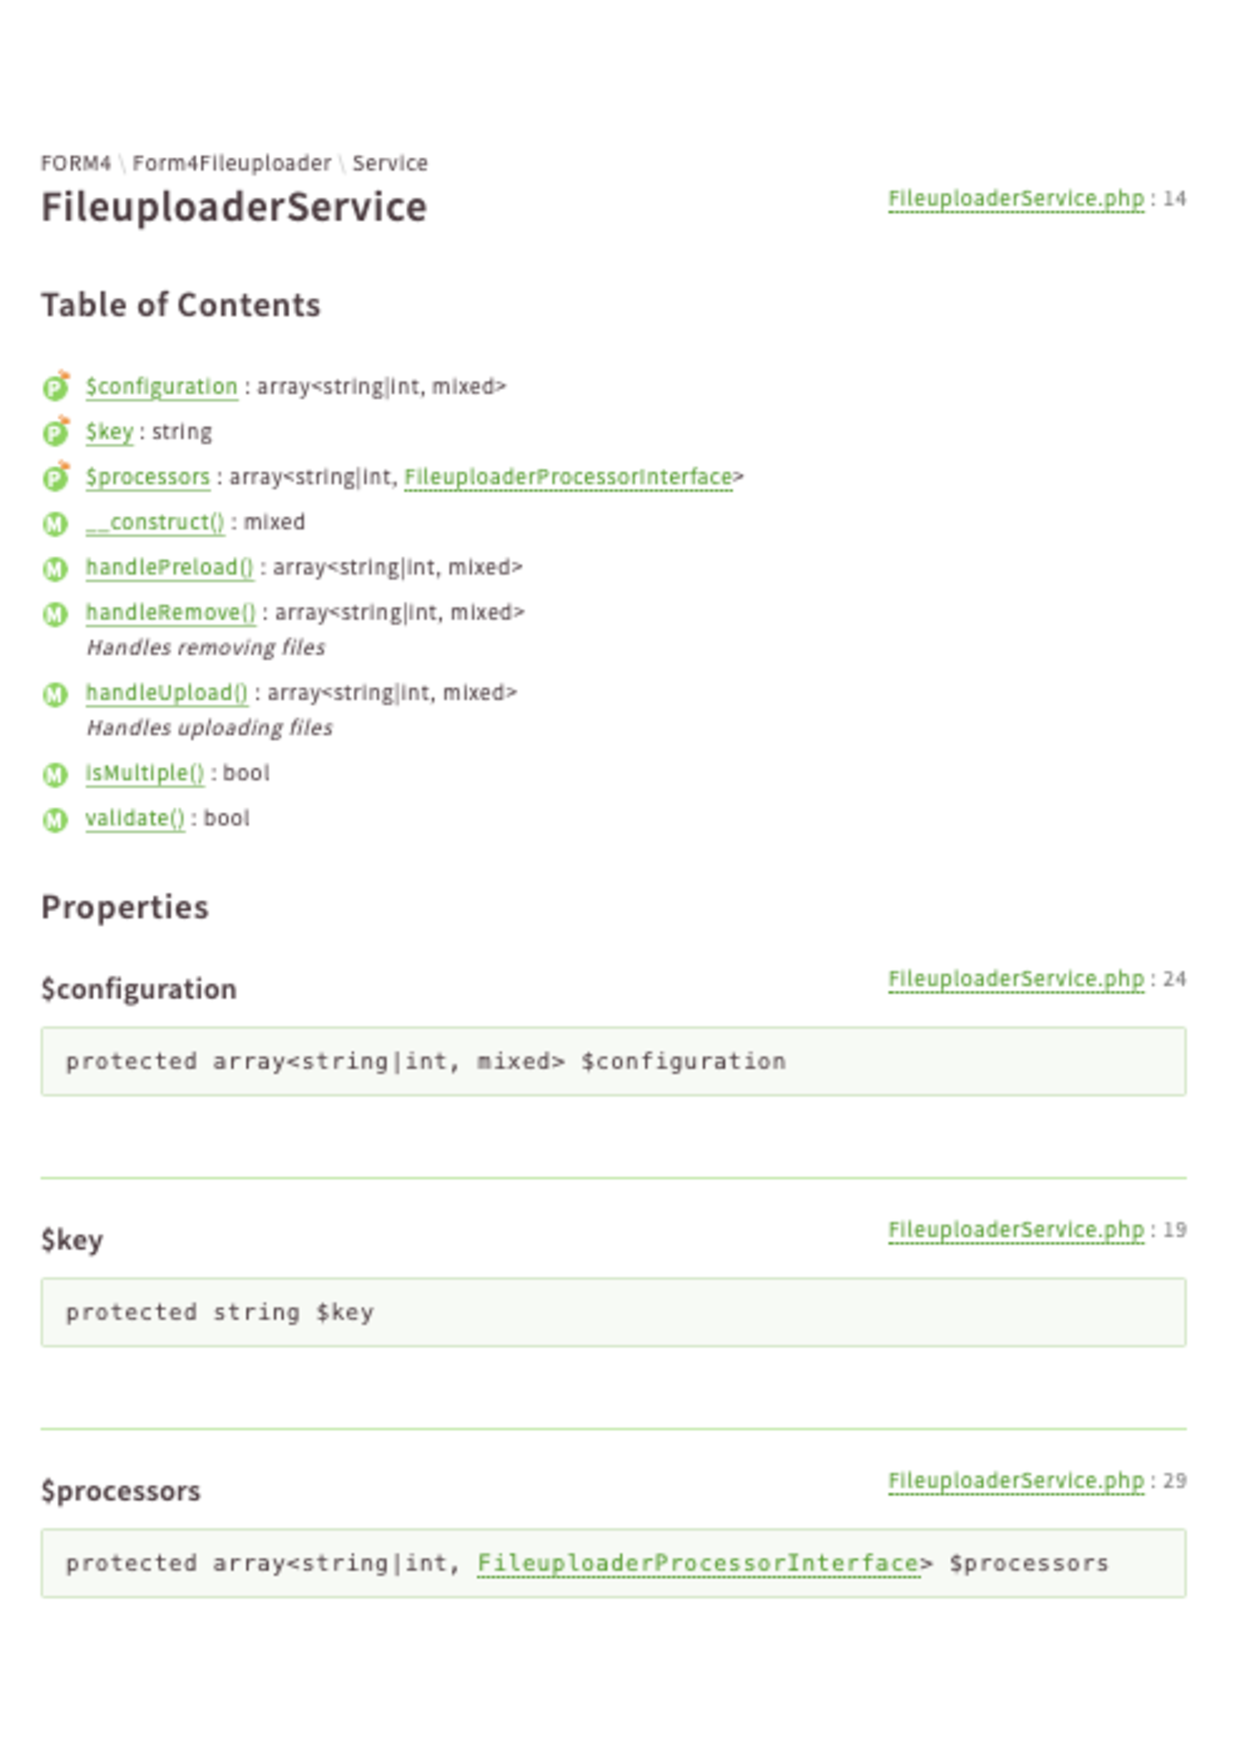
\includegraphics[page=1, width=0.9\textwidth]{doc.pdf}

\includegraphics[page=2, width=0.9\textwidth]{doc.pdf}
\end{center}

\clearpage
\subsection{Testfall und sein Aufruf auf der Konsole}
\label{app:Test}
\lstinputlisting[language=php, caption={Testfall in PHP}]{Listings/tests.php}
\clearpage
\begin{figure}[htb]
\centering
\includegraphicsKeepAspectRatio{testcase.jpg}{1}
\caption{Aufruf des Testfalls auf der Konsole}
\end{figure}


\subsection{Klasse: ComparedNaturalModuleInformation}
\label{app:CNMI}
Kommentare und simple Getter/Setter werden nicht angezeigt.
\lstinputlisting[language=php, caption={Klasse: ComparedNaturalModuleInformation}]{Listings/cnmi.php}
\clearpage

\subsection{Klassendiagramm}
\label{app:Klassendiagramm}
Klassendiagramme und weitere \acs{UML}-Diagramme kann man auch direkt mit \LaTeX{} zeichnen, siehe \zB \url{http://metauml.sourceforge.net/old/class-diagram.html}.
\begin{figure}[htb]
\centering
\includegraphicsKeepAspectRatio{Klassendiagramm.pdf}{1}
\caption{Klassendiagramm}
\end{figure}
\clearpage

\subsection{Benutzerdokumentation}
\label{app:BenutzerDoku}
Ausschnitt aus der Benutzerdokumentation:

\begin{table}[htb]
\begin{tabularx}{\textwidth}{cXX}
\rowcolor{heading}\textbf{Symbol} & \textbf{Bedeutung global} & \textbf{Bedeutung einzeln} \\
\includegraphicstotab[]{weather-clear.png} & Alle Module weisen den gleichen Stand auf. & Das Modul ist auf dem gleichen Stand wie das Modul auf der vorherigen Umgebung. \\
\rowcolor{odd}\includegraphicstotab[]{weather-clear-night.png} & Es existieren keine Module (fachlich nicht möglich). & Weder auf der aktuellen noch auf der vorherigen Umgebung sind Module angelegt. Es kann also auch nichts übertragen werden. \\
\includegraphicstotab[]{weather-few-clouds-night.png} & Ein Modul muss durch das Übertragen von der vorherigen Umgebung erstellt werden. & Das Modul der vorherigen Umgebung kann übertragen werden, auf dieser Umgebung ist noch kein Modul vorhanden. \\
\rowcolor{odd}\includegraphicstotab[]{weather-few-clouds.png} & Auf einer vorherigen Umgebung gibt es ein Modul, welches übertragen werden kann, um das nächste zu aktualisieren. & Das Modul der vorherigen Umgebung kann übertragen werden um dieses zu aktualisieren. \\
\includegraphicstotab[]{weather-storm.png} & Ein Modul auf einer Umgebung wurde entgegen des Entwicklungsprozesses gespeichert. & Das aktuelle Modul ist neuer als das Modul auf der vorherigen Umgebung oder die vorherige Umgebung wurde übersprungen. \\
\end{tabularx}
\end{table}




% Quellen ---------------------------------------------------------------------
\clearpage
\pagenumbering{roman}
% !TEX root = Projektdokumentation.tex
\section{Quellenangaben}

Leitfaden zur IHK-Abschlussprüfung Fachinformatiker/-in Anwendungsentwicklung

LaTeX Vorlage: \url{https://github.com/StefanMacke/latex-vorlage-fiae}

The TYPO3 Project and Community: \url{https://typo3.org/}

What is a transcompiler?: \url{https://www.computerhope.com/jargon/t/transcompiler.htm}

ECMAScript 2015 - ES6: \url{https://www.w3schools.com/js/js_es6.asp}

TypeScript: \url{https://www.typescriptlang.org/}

Babel: \url{https://babeljs.io/}

README - MobX: \url{https://mobx.js.org/README.html}

MobX Tutorial: \url{https://mobx.js.org/getting-started}

Functional reactive programming: \url{https://www.it-economics.de/software-architektur/2019-06/functional-reactive-programming-frp-mehr-als-nur-datenstroeme-und-lambdas-1}


\end{document}
